\prob
{
    For $r \geq 2$, consider an $r\times (2^r -1)$ matrix $A_r$ whose columns are all of the non-zero vectors in
    $V(r,2)$. The vectors in the orthogonal subspace of $\mathcal{R}(A_r)$ from the binary Hamming code $H_r$ is only
    determined up to a permutation of the coordinates. Show that:
    \begin{enumerate}[label=(\roman*)]
        \item $H_3$ equals the row space of the following matrix over $GF(2)$.
                \begin{center}
                    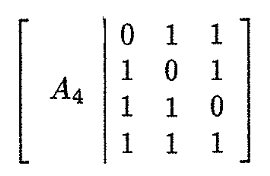
\includegraphics[width=4cm]{Test3/Problem6/matrix.png}
                \end{center}\pn
        \item $H_r$ has dimension $2^r -r - 1$.
        \item There is a partition of $V(2^r - 1, 2)$ into $m$ classes where $m$ is the number of vectors in $H_r$ and
              each class contains a unique member $v$ of $H_r$ together with all members of $V(2^r - 1, 2)$ that differ from $v$ in
              exactly one coordinate.
    \end{enumerate}
}